% % %
%
%	- Introduction- 
%
% % %
\chapter{Introduction}
\label{cha:introduction}
The introduction of a thesis usually contains the motivation for the topic, the problem statement (see section \ref{sec:introduction:problemstatement}), a description of the  contribution / results of the thesis (see section \ref{sec:introduction:objective}), and a short description of the structure of the thesis (see section \ref{sec:introduction:structure}).\\


% Example referencing figures
A figure is always referenced in text. See vor example figure \ref{fig:rbf-net}. \\ %linebreak

% Referencing chapters, sections, ...
Whole chapters are referenced using  Chapter \ref{cha:introduction}, subsections using subsection \ref{sec:introduction:problemstatement}. \\ %linebreak

% Example referencing literature
Statement originating from the literature receive a reference at the end of the sentence \cite{schwenker2001three}. 
% Figure of a 2 layer RBF network
\begin{figure}[htp]
\begin{center}
  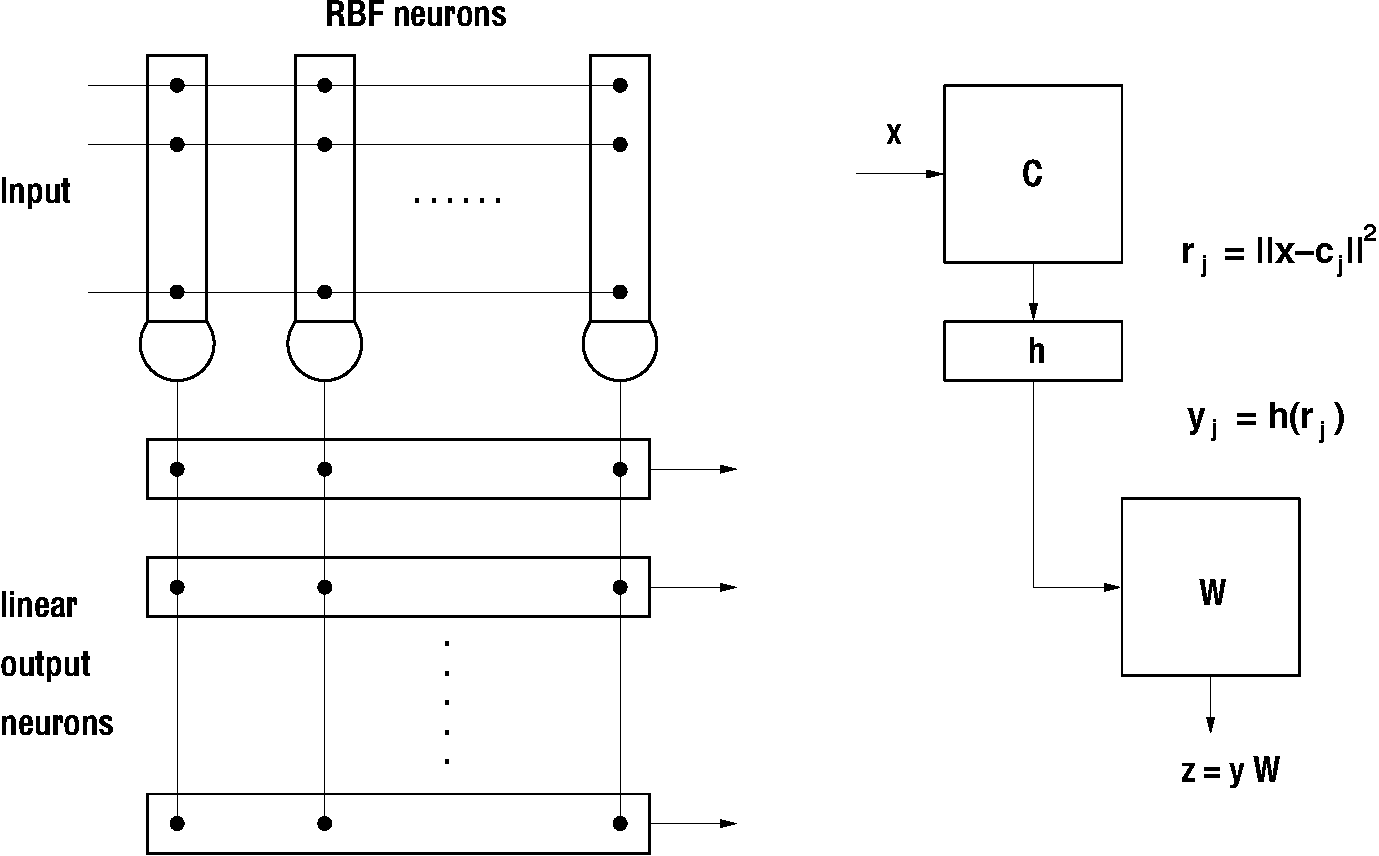
\includegraphics[width=0.99\linewidth]{rbf-net} %pdf, jpg, png...
  \caption{A simple two layer radial basis function network}
  \label{fig:rbf-net}
\end{center}
\end{figure}

% Section: problem statement
\section{Problem statement}
\label{sec:introduction:problemstatement}
The problem statement of your thesis goes here!


% Section: objective
\section{Contributions and results}
\label{sec:introduction:objective}
Describe contributions and results here!


% Section: structure of the thesis
\section{Structure of the thesis}
\label{sec:introduction:structure}
Explain the structure of your thesis here!

